\chapter{Проектирование приложения} \label{chapt2}

\section{Общий вид приложения} \label{sect2_1}

Чтобы представить общий вид приложения следует вернуться к поставленным задачам:

\begin{itemize}
  \item Переключение между различными ролями в RTK системе
  \item Возможность изменять настройки основных режимов работы
  \item Работа с конфигурационными файлами(создание, копирование, удаление)
  \item Отображение статуса системы - текущие координаты, качество решения
  \item График уровней приема сигнала спутников
  \item Cписок логов ГНСС данных с возможностью их скачать
  \item Возможность сконвертировать логи ГНСС данных в формат RINEX
\end{itemize}

Следует разбить эти задачи на группы. К примеру, цель одних - отображение результата работы RTKLIB, цель других - изменение настроек. Также есть вспомогательные, но необходимые для нормальный работы задачи, такие как хранение, организация и скачивание логов. К задачам отображения следует отнести статус системы и график уровней приема спутников, очень полезный при установке антенны. К настройкам - переключение между ролями базы и ровера и, собственно, настройки этих самых ролей.

\clearpage

Как было видно из предыдущей главы, разбиение веб-страницы на тематические разделы - ход, на который пошла как большая компания, так и open source проект. Здесь это также представляется удобным ходом. Для разграничения областей можно использовать стандартные для мобильных приложений вкладки.

\begin{figure}[ht]
  \center
  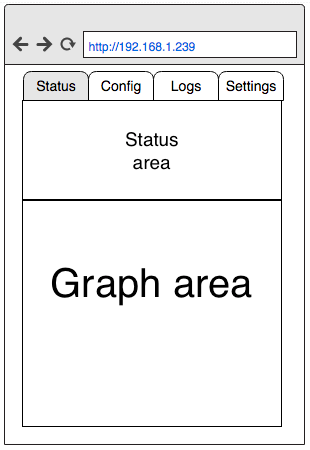
\includegraphics [scale=0.5] {General_mockup}
  \caption{Навигация внутри приложения}
  \label{img:latex}
\end{figure}

\clearpage

\section{Вкладки приложения} \label{sect2_2}

\subsection{Status} \label{subsect2_2_1}

В статус следует поставить информацию о координате, RTK режиме, статусе RTK решениия. Кроме этого на один экран можно уместить и график с уровнями приема спутников. Примерный вид можно представить в таком виде:

\begin{figure}[ht]
  \center
  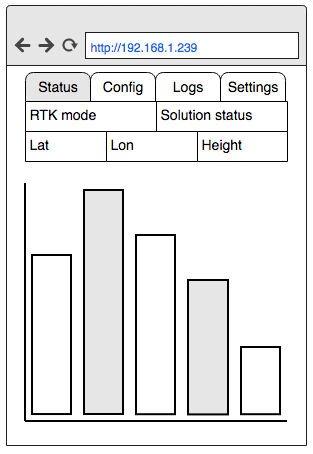
\includegraphics [scale=0.5] {Status_mockup}
  \caption{Статус приемника}
  \label{img:latex}
\end{figure}

\clearpage

\subsection{Config} \label{subsect2_2_2}

Вкладка конфигурации должна содержать возможность переключаться с базы на ровер и обратно. Кроме этого, нужно отображать настройки соответствующего режима. В случае с ровером должен быть выбор, какой конфигурационный файл использовать.

\begin{figure}[ht]
  \center
  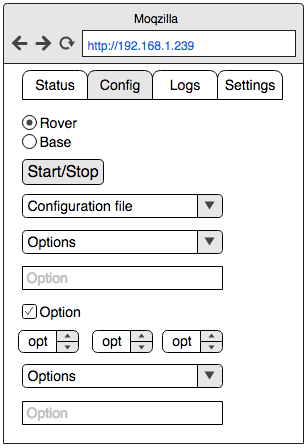
\includegraphics [scale=0.5] {Config_mockup}
  \caption{Конфигурация}
  \label{img:latex}
\end{figure}

\clearpage

\subsection{Logs} \label{subsect2_2_3}

Вкладка с логами будет содержать список логов. Удобнее всего логи сортировать по дате, но в обратном порядке. По нажатию на элемент такого списка, будет начинаться загрузка. Каждый элемент списка может содержать информацию о времени начала лога, формате и размере.

\begin{figure}[ht]
  \center
  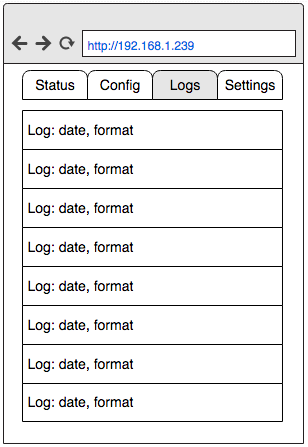
\includegraphics [scale=0.5] {Logs_mockup}
  \caption{Логи на устройстве}
  \label{img:latex}
\end{figure}

\clearpage

\subsection{Settings} \label{subsect2_2_4}

Здесь будут находиться настройки самого приложения: указание текущей версии и возможность обновления, выбор версии формата RINEX для конвертации логов, кнопка перезагрузки устройства.

\begin{figure}[ht]
  \center
  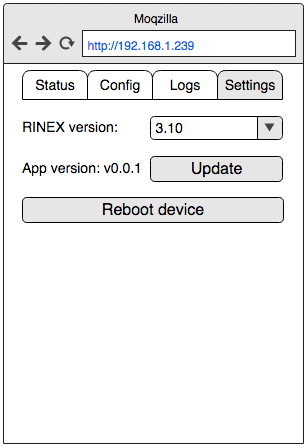
\includegraphics [scale=0.5] {Settings_mockup}
  \caption{Настройки приложения}
  \label{img:latex}
\end{figure}

\clearpage

\section{Взаимодействие с RTKLIB} \label{sect2_3}

Одним из сложных вопросов, которые следует решить при проектировании приложения - как наладить обмен информацией с программами RTKLIB. Существуют следующие варианты решения проблемы:

\begin{enumerate}
  \item Дописать приложение и серверную часть на языке C
  \item Дописать в RTKLIB передачу данных в механизм IPC уровня операционной системы и читать полезную информацию из стороннего приложения-сервера
  \item Запускать приложения RTKLIB в контолируемом контейнере, имитирующем запуск человеком в терминале
\end{enumerate}

Дело в том, приложения пакета написаны на C, а это не самый подходящий язык для написания веб-приложения. Существуют вэб фрэймворки и для языка C, но это скорее исключения из правил.

Еще одним важным аспектом, который нельзя не принять во внимание - общий стиль реализации проекта. Дело в том, что RTKLIB написан излишне сложно. Вот, например, выдержка из кода проекта:

\lstinputlisting[
  label={listings:rtklib_code_snippet},
  caption={Пример исходного кода RTKLIB},
  style={java}
]
{src/rtklib_code_snippet.c}

Все это наталкивает на мысль, что наиболее простым и наиболее надежным способом работы с приложениями RTKLIB будет не вмешиваться в код проекта и не дописывать новую функциональность прямо в код приложений, а сделать обертку вокруг собранных исполняемых файлов. Под «оберткой» следует понимать запуск приложения в контролируемой среде, чтение и парсинг стандартного вывода, запись команд в стандартный ввод. Это позволит:

\begin{itemize}
  \item Не вмешиваться в сложную внутреннюю структуру приложения, рискуя что-то нарушить
  \item Сохранить совместимость с новыми версиями RTKLIB, даже при серьезных изменения кодовой базы
  \item Писать веб-приложение на более подходящем для этого языке
  \item Не добавлять никакие дополнительные механизмы IPC в RTKLIB
\end{itemize}

% \clearpage

\section{Общая архитектура и выбор инструментов разработки} \label{sect2_4}

Так как основа всего проекта - веб-приложение, следует выбрать язык с популярным и функциональным фрэймворком для веб-разработки. Также, языку требуется наличие библиотеки для запуска внешних программ в контролируемом контейнере, как описано в предыдущей главе. Не следует забывать о том, что приложение будет запускаться на встраиваемом модуле с ограниченными параметрами производительности. Эти черты пересекаются в языке Python, дополненном библиотекой Pexpect и фрэймворком Flask.

Чтобы добиться ощущения мобильного приложения, можно использовать такую технику: сделать само приложение одностраничным(реализовав вкладки внутри одной из страниц), а любые взаимодействия с сервером, кроме загрузки самой страницы, проводить через технологию WebSockets. Поддержка веб-сокетов реализована с помощью Javascript библиотеки Socket.io со стороны клиента и расширением flask-socketio \cite{flask-socketio-docs} для сервера Flask.

При создании веб-страницы, помимо библиотеки для работы с веб сокетами, можно ограничиться стандартными инструментами - HTML, библиотеки jQuery для манипуляций над элементами DOM. Также, для адаптивности страницы нужен подходящий набор элементов пользовательского интерфейса для создания самой страницы. Такой UI фрэймворк обеспечит работу приложения для практически любого браузера, на экранах самых разных размеров. Был выбран jQuery Mobile, позволящий модифицировать стандартные элементы HTML страницы добавлением правильных свойств.

\clearpage

Результат работы, общий план архитектуры приложения можно увидеть на рисунке 2.6.
\begin{figure}[ht]
  \center
  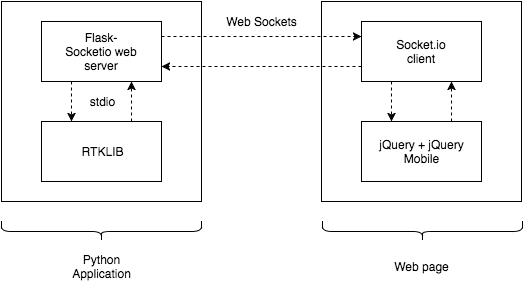
\includegraphics [scale=0.6] {App_architecture}
  \caption{Общий план архитектура приложения}
  \label{img:latex}
\end{figure}














